\documentclass[sigconf]{acmart}
% ===== Don't touch this :) ======
\settopmatter{printacmref=false} % Removes citation information below abstract
\renewcommand\footnotetextcopyrightpermission[1]{} % removes footnote with conference information in first column
\renewcommand\footnotetextauthorsaddresses[1]{}
\pagestyle{plain} % removes running headers
\graphicspath{ {./images/} }
% ================================
\usepackage{graphicx}
\usepackage{indentfirst}
\usepackage{float}
\usepackage{hyperref}
\usepackage{color}

\begin{document}
    \title{CS561 : Performance Comparison between LSM-Trees and B+-Trees}

    \author{Richard Andreas}
    \affiliation{%
        \institution{ra7296@bu.edu}
    }
    \author{Jingyu Su}
    \affiliation{%
        \institution{jingyusu@bu.edu}
    }
    \author{Xingkun Yin}
    \affiliation{%
        \institution{yinxingk@bu.edu}
    }

    \begin{abstract}
        In this paper, we explore the the design space of key-value stores that utilize the Log-Structured merge-tree (LSM-Tree) structure. More specifically, we have implemented a base version of the LSM-Tree that have been explored in previous work in order to get a better understanding of the basic knowledge of it. We decided to compare between performance of our design to another data structure (B+-tree), to see which data structure performs better based on different workloads and operations. Instrutions to compilationare and running are in the README.md of the repository of this project: \href{https://github.com/randreas/LSM_Tree_Repo}{\color{blue}{LSM Tree}}.
    \end{abstract}

    \maketitle

% =============================================================================
    \section{Introduction}
% =============================================================================

    \subsection{Motivation}


    Log-Structured merge-tree (LSM-trees) are one of the most commonly used data structures for persistent storage of key-value entries. LSM-tree based storages are in use in several modern key-value stores including RocksDB at
    Facebook, LevelDB and BigTable at Google, bLSM and cLSM at Yahoo!, Cassandra
    and HBase at Apache.

    In addition to LSM Trees, B+ trees is another common data structure for key-value entries. A B+-tree is an index data structure that stores data pointers only in leaf nodes, and only pivot pivot pointers in the internal nodes. Additiaonlly, the leaf nodes are also linked to provide ordered access to the records,

    \subsection{Problem Statement}

    When choosing which data structure to use for indexing and searching, we typically would choose between these 2 data structures as they are widely known and have superior performance compared to the rest. However, this brings us to the next question, how do we pick between these two. In our paper, we will experiment on both data structures with various workloads and compare their performance in 4 operations: insert, delete, point scan, range scan. We expect to discover a pattern on the performance differences between the two indexes, and answer the question.


% =============================================================================
    \section{Background}
% =============================================================================

    In this section, we will be presenting the background of LSM-trees, by discussing the basic structure of LSM-trees used in today's storage systems.

    \subsection{Basic Structure}
    Today's LSM-Tree implementation applies updates out-of-place to reduce Random I/Os. All incoming writes are appended into a memory buffer. An insert or update operation simply adds a new entry, while a delete operation adds a graveyard pointer indicating the entry has been deleted.

    A query over an LSM-Tree has to search multiple components to find the latest version of each key. A point look up query, which fetches the value of a specific key, simply search all components one by one, from newest to oldest, and stops immediately after the first match is found. A range scan can search all components at the same time, feeding the search results into a query.

    As components or data blocks accumulate over time, the query performance of an LSM-Tree tends to degrade since more components must be examined. These components are merged to reduce the total number of components. There are two types of merge policies, leveling and tiering. Both policies organize components or data blocks, into logical levels (or tiers) and controlled by a size ratio of T. Each component is labeled with its key range.

    In Leveling, each level only maintains one component, but the component at level L is T time larger than the component at level L-1. As a result, the component at level L will be merged multiple times with incoming components at level L-1 until it feels up, and it will then be merged into level L+1.

    In Tiering merge policy maintains up to T components per level. When level L is full, its T components are merged together into a new component at level L+1. If level L is already the configured maximum level, then the resulting component remains at level L. Two components at level L-1 are merged together to form a new component/data block at level L.\\
    \begin{figure}[H]
        \centering
        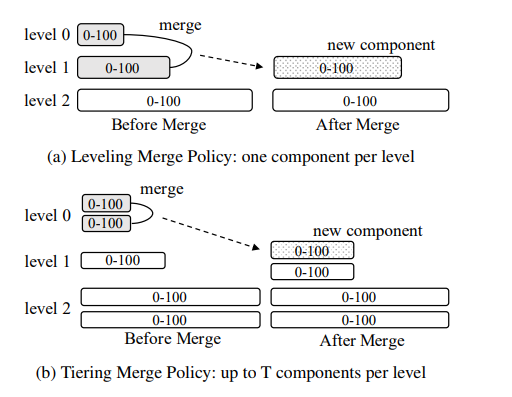
\includegraphics[width=0.5\textwidth]{MergingStrategies.PNG}
        \caption{LSM Tree merge policies}
        \label{Fig.main2}
    \end{figure}
% =============================================================================
    \section{Architecture}
% =============================================================================
    In this section, we will analyze the main components of our LSM-Tree Architecture.
    \subsection{Tuple}
    Tuples are the units of data stored in a LSM-tree. In our implementation, a tuple consists of a key, a value, and an identifier of the type of the operation.

    \subsection{Run}
    A run is the form of a block of data in a level of LSM tree in the LSM tree when it is actual been read into memory. It contains the actual data.

    \subsection{Buffer}
    Operation log entries of the LSM tree goes directly into the buffer. Buffer in this project is an instance of Run. It has a fixed size, the same size as the blocks on the first level of the tree and it is the first data to look into when query. When the buffer if full, it is swapped into level 1 and the compaction process of this LSM tree begins.

    \subsection{Bloom Filters}
    Bloom Filters are an essential component of the LSM-Tree. The concept of a bloom filter is suggested as the main mechanism to avoid unnecessary level accesses. Queries first check the bloom filter, if the result is positive, then it checks the level, otherwise check a lower level or return not found if at bottom level. The main drawback is the possibility of giving a false positive result.

    \subsection{Fence Pointers}
    Fence Pointers are the limits of the virtual blocks of data. By implementing fence pointers, we are do not have to access every single data entry during scanning or point searching. We implement fence pointers in the form of zonemaps. By checking the min/max values in each fence pointer, this reduces the time it takes for searching as we ignore blocks of data that do not meet the requirements.

    \subsection{Levels}
    Levels are the core in LSM trees as they contain actual data entries. Our implementation of levels contain "FileMeta" objects, each of the FileMeta objects contain information necessary to access the correct data file on disk. Upon query, the LSM tree deserializes the data file with the information in the corresponding FileMeta, instantiates an Run object accordingly, and either return the result of query or modify the file. Run objects are destructed when query finishes.

    \subsection{FileMeta}
    FileMeta corresponds to a block of data in a level. It is on persistent storage, in the case of this project, a local file. Filedata store the metadata of the block, including the path to the file, the upper bound and the lower bounding of this file. When LSM compact severl blocks into one single block, the corresponding filemeta are combined into a new file meta as well and the new filemeta contain all the metadata about the new block.

    \subsection{Testing}
    We tested the correctness of our implementation using a dataset created by ourselves. Will test more intensively in the future.

    \subsection{Benchmark Explanations}

    We used the data.wl and workload.wl files to test the correctness of our program. The data set covers the operation supported for now, and makes sure that the number of entries in the LSM tree is big enough to overflow the buffer, in order to trigger merge and tiering mechanism.


% =============================================================================
    \section{Results}
% =============================================================================
    Will be updated after further benchmarking.

    \begin{figure}[ht]
        \includegraphics[width=3cm]{example-image-a}
        \caption{Example figure here}
        \label{fig:filler}
    \end{figure}

    \begin{table}[H]
        \caption{An example table}
        \label{tab:ex}
        \centering

        \begin{tabular}{c |c c c c c}
            \hline\hline
            & Col A & Col B \\
            \hline
            Row A & val 1 & val a \\
            Row B & val 2 & val b \\
            Row C & val 3 & val c \\
            \hline
        \end{tabular}
    \end{table}

    You can also reference your old figures (Figure \ref{fig:filler}) and tables
    (Table \ref{tab:ex})

% =============================================================================
    \section{Current Progress So Far}
% =============================================================================

    We have finished coding the basic features of the LSM-Tree: Fence Pointers, Leveling, Buffers, Bloom Filters and basic operations such as Insert and point query. Our prototype works with a basic workload and is able to run smoothly.

% =============================================================================
    \section{Future work to be done}
% =============================================================================

    We will change the low level disk file format from current easy-but-slow .txt file storing strings to binary files that are both temporal and spatial efficient.

    We will finish up the remaining the operations: Delete and Range Scan.

    We will start working on is testing the prototype with a bigger workload and various levels of unsorted-ness to measure the performance of our implementation.


    We will use a provided implementation of a B+ tree, and run the same the tests that we have run on the LSM tree, to ensure fair testing between both data structures.

    Setting up a Virtual Machine will be part of this process and we can run the experiments on it.

% =============================================================================
    \section{Conclusion}
% =============================================================================

    We will have a conclusion after future benchmarking.

% reference
        {
        \bibliographystyle{ACM-Reference-Format}
        \bibliography{biblio}

        [1] Chen Luo, Michael J. Carey. LSM-based storage techniques: a survey. VLDB J.29(1): 393-418 (2020)

        [2] Niv Dayan, Manos Athanassoulis, Stratos Idreos. Monkey: Optimal Navigable
        Key-Value Store. SIGMOD Conference 2017: 79-94

        [3] Patrick E. O'Neil, Edward Cheng, Dieter Gawlick, Elizabeth J. O'Neil. The LogStructured Merge-Tree (LSM-Tree). Acta Inf. 33(4): 351-385 (1996)
    }

\end{document}
